\documentclass{beamer}
\usepackage[spanish]{babel}
\selectlanguage{spanish}
\usepackage[utf8]{inputenc}
\usepackage{hyperref}
\usepackage{graphicx}
\usepackage{float}


\usetheme{Frankfurt}
\usecolortheme{whale}

\title{Conceptos de Git}
\author{Emmanuel Arias \href{mailto:emmanuelarias30@gmail.com}{emmanuelarias30@gmail.com}}
\date{}
\begin{document}
\begin{frame}[plain]
    \maketitle
\end{frame}

\begin{frame}
	\Huge Procesos o etapas de Git
\end{frame}

\begin{frame}{Proceso o etapas de Git}
	\begin{figure}
		\centering
		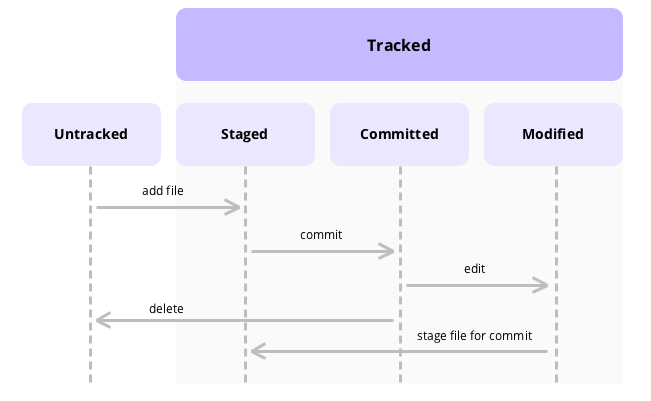
\includegraphics[width=1\linewidth]{img/stages}
		\label{fig:stages}
	\end{figure}
\end{frame}

\begin{frame}{Procesos o etapas de Git}
\begin{itemize}
	\item Untracked: Se refiere a los archivos que no están en stagging ni tampoco en la base de datos. Son archivos nuevos que no están registrados.
	\item Stagged: Es la versión actual de tus archivos y/o proyecto. Es lo que en un futuro se convertirá en parte "freezada" del proyecto o software, es decir cuando ya pase por un commit.
	En este momento el archivo o cambio no está en el repositorio todavía, si no que está próximamente a estarlo.
\end{itemize}
\end{frame}

\begin{frame}
	 \begin{itemize}
		\item Modified: Archivos que fueron modificados en el respositorio y por lo tanto, no es la versión que está almacenada en el repositorio. Para que este cambio llegue al respositorio, primero debe pasar por Stagged y recien puede ir a la base de datos.
	 	\item Commited o Base de datos o  Repositorio: Significa que estos archivos ya están en la base de datos. Es decir están almacenados en el repositorio.
	 \end{itemize}
\end{frame}

\begin{frame}
   \Huge Git Internals
\end{frame}

\begin{frame}{Git Internals}
	\begin{itemize}
		\item En git los archivos se almacenan en archivos \textbf{blobs} (binary large objects)
		\item La ventaja de usar estos Blob y un archivo normal es que estos últimos guardan metadata. En cambio los Blobs es solo contenido.
		\item Cada blob es identificado por un código has SHA-1. 
		\item En Git cada directorio o carpeta se lo llama Tree. También identificado por un hash SHA-1.
	\end{itemize}
\end{frame}

\begin{frame}{Git Internals}
	\begin{figure}
		\centering
		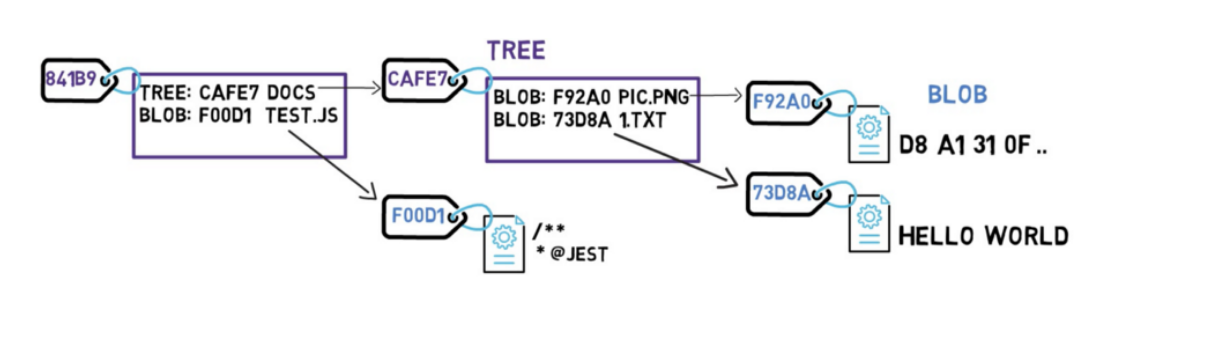
\includegraphics[width=1\linewidth]{img/tree-blobs}
		\label{fig:tree-blobs}
	\end{figure}
\end{frame}

\begin{frame}{Git Internals - Commit}
\begin{figure}
	\centering
	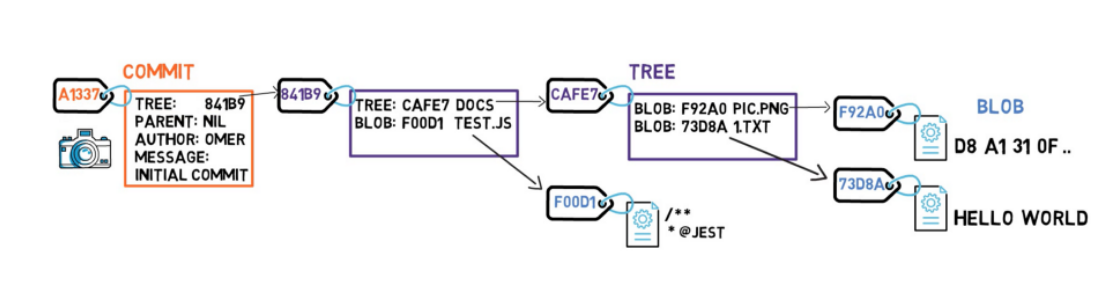
\includegraphics[width=1\linewidth]{img/tree-blobs1}
	\label{fig:tree-blobs1}
\end{figure}
\end{frame}

\begin{frame}[plain]{Links interesantes}
	\begin{itemize}
		\item \href{https://git-scm.com/book/es/v2/Los-entresijos-internos-de-Git-Los-objetos-Git}{Los objetos de Git}
		\item \href{https://www.bitdegree.org/learn/git-cheat-sheet}{Git cheat sheet}
		\item \href{https://almasumfahim.com/git-stages/}{Git stages}
	\end{itemize}
\end{frame}

\end{document}
